\documentclass[11pt,aspectratio=169]{beamer}

\usepackage{slides}
\usepackage{soul}
\usepackage{pdfpc}
\usepackage{ebproof}
\usepackage{bigdelim}
\usepackage{booktabs}
\usepackage{listings}
\usepackage{tcolorbox}
\usepackage{tabularx}
\usepackage{tikz}
\usepackage{xspace}
\usepackage[T1]{fontenc}
\usepackage[utf8]{inputenc}
\usepackage[symbol]{footmisc}
\usepackage[noend]{algpseudocode}
\usepackage[
    backend    = biber,
    style      = alphabetic,
    giveninits = true,
    maxnames   = 16,
    minnames   = 16,
]{biblatex}

\addbibresource{./references.bib}

\usetikzlibrary{
    positioning,
    shapes.symbols,
    shadows,
    arrows,
    calc
}

\newcommand{\senc}{\text{senc}}
\newcommand{\msg}{\text{msg}}
\newcommand{\nonce}{\text{nonce}}
\newcommand{\KDF}{\text{KDF}}
\newcommand{\key}{\text{key}}

\newcommand{\Tamarin}[1]{\textsc{Tamarin}\xspace}

%% Print: [#1] -[#2]-> [#3]
\newcommand{\MSR}[3]{#1 -\hspace{-4pt}[\hspace{5pt} #2 \hspace{4pt}]\hspace{-4.6pt}\rightarrow #3}
%% Print: -[#1]->
\newcommand{\ActionFact}[1]{-\hspace{-4pt}[\hspace{5pt} #1 \hspace{4pt}]\hspace{-4.6pt}\rightarrow}
%% Print: ~
\newcommand{\tildelow}{\raisebox{0.5ex}{\texttildelow}}
%% Print: ^
\newcommand{\pow}{\textasciicircum{}}
%% Highlight text in overlay
\newcommand{\althl}[2][2]{\alt<#1>{\hl{#2}}{#2}}

%% Sticky notes to represent facts
\definecolor{StickyNoteYellow}{RGB}{241,239,161}
\definecolor{StickyNoteRed}{RGB}{255,167,169}
\definecolor{StickyNoteGreen}{RGB}{148,199,146}
\definecolor{StickyNoteBlue}{RGB}{167,229,241}
\NewDocumentCommand{\StickyNote}{O{StickyNoteYellow}O{1cm}m}{%
    \begin{tikzpicture}
        \node[
            drop shadow={
                shadow xshift = 2pt,
                shadow yshift = -4pt,
            },
            xslant = -0.1,
            yslant = 0.1,
            draw   = black,
            fill   = #1,
            text   = black,
        ] {\parbox[t][#2][c]{#2}{\centering#3}};
    \end{tikzpicture}
}

%% Colors for terms and facts
\definecolor{TermBlue}{HTML}{1C377D}
\definecolor{FactPurple}{HTML}{7C3655}

\newcommand{\term}[1]{\textcolor{TermBlue}{#1}}
\newcommand{\Term}[1]{\textcolor{TermBlue}{#1}}
\newcommand{\Fact}[1]{\textcolor{FactPurple}{#1}}

%% Other colors
\definecolor{AdversaryRed}{HTML}{DA3B26}

%% Listings
\lstset{escapeinside={(*@}{@*)}}
\lstset{numberstyle=\tiny}

\definecolor{TamarinBlue}{RGB}{42,0,255}
\definecolor{TamarinGreen}{RGB}{48,110,32}
\definecolor{TamarinPurple}{RGB}{175,36,67}

\lstdefinestyle{tamarin}{
    basicstyle    = \linespread{0.75}\footnotesize\ttfamily,
    extendedchars = true,
    tabsize       = 2,
    columns       = fixed,
    numbers       = none,
    breaklines    = true,
    literate      = {~}{{\raisebox{0.5ex}{\texttildelow}}}{1},
    morekeywords  = {theory, builtins, restriction, equations, functions, rule,
                     let, in, lemma, All, Ex, not, predicates, begin, end},
    keywordstyle  = \color{TamarinPurple},
    morecomment   = [l]{//},
    morecomment   = [s]{/*}{*/},
    commentstyle  = \color{TamarinGreen},
    xleftmargin   = 0mm,
    upquote       = true,
    morestring    = *[b]",
    showstringspaces = false
}

\lstdefinestyle{tactic}{
    basicstyle    = \linespread{0.75}\footnotesize\ttfamily,
    extendedchars = true,
    tabsize       = 2,
    columns       = fixed,
    numbers       = none,
    breaklines    = true,
    literate      = {~}{{\raisebox{0.5ex}{\texttildelow}}}{1},
    alsoletter    = :,
    morekeywords  = {tactic:, presort:, prio:, deprio:},
    keywordstyle  = \color{TamarinPurple},
    morecomment   = [l]{//},
    morecomment   = [s]{/*}{*/},
    commentstyle  = \color{TamarinGreen},
    xleftmargin   = 0mm,
    upquote       = true,
    morestring    = *[b]",
}

\lstdefinestyle{oracle}{
    basicstyle    = \linespread{0.75}\footnotesize\ttfamily,
    extendedchars = true,
    tabsize       = 2,
    columns       = fixed,
    numbers       = none,
    breaklines    = true,
    literate      = {~}{{\raisebox{0.5ex}{\texttildelow}}}{1},
    morecomment   = [l]{\#},
    morekeywords  = {import, for, in, if, elif},
    keywordstyle  = \color{TamarinPurple},
    commentstyle  = \color{TamarinGreen},
    xleftmargin   = 0mm,
    upquote       = true,
}

\definecolor{ProVerifGreen}{RGB}{48,110,32}
\definecolor{ProVerifBlue}{RGB}{64,112,161}

\lstdefinestyle{proverif}{
    basicstyle    = \linespread{0.75}\footnotesize\ttfamily,
    extendedchars = true,
    tabsize       = 2,
    columns       = fixed,
    numbers       = none,
    breaklines    = true,
    literate      = {~}{{\raisebox{0.5ex}{\texttildelow}}}{1},
    morecomment   = [s]{(*}{*)},
    commentstyle  = \color{ProVerifGreen},
    keywordstyle  = \color{ProVerifBlue},
    morekeywords  = {in, if, event, new, let, out},
    xleftmargin   = 0mm,
}

\definecolor{proofTreeBlue}{HTML}{2639B0}
\definecolor{proofTreeRed}{HTML}{921C12}

\lstdefinestyle{prooftree}{
    basicstyle    = \linespread{0.8}\footnotesize\fontfamily{pcr}\selectfont,
    extendedchars = true,
    tabsize       = 2,
    columns       = fixed,
    numbers       = left,
    breaklines    = true,
    literate      = {~}{{\raisebox{0.5ex}{\texttildelow}}}{1},
    keywords      = [1]{lemma, case, next, qed, by, end, Diff-Lemmas},
    keywordstyle  = [1]\color{black}\bfseries,
    keywords      = [2]{simplify, solve, sorry, contradiction, induction,
                        autoprove, rule-equivalence},
    keywordstyle  = [2]\color{proofTreeBlue}\bfseries,
    keywords      = [3]{@, \|, <, \^},
    keywordstyle  = [3]\color{proofTreeRed},
    alsoletter    = @\|<\^-,
    moredelim     = **[is][{\color{proofTreeBlue}}]{<<}{>>},
    xleftmargin   = 0mm,
    upquote       = true,
    morestring    = *[b]",
}

%% Color boxes
\definecolor{ColorBoxBlue}{HTML}{1C377D}
\tcbset{
    colback      = white,
    colframe     = black,
    fonttitle    = \bfseries,
    coltitle     = white,
    colbacktitle = ColorBoxBlue,
    boxrule      = 1pt
}

%% Vertical separator for frames
\newcommand<>{\vsep}{
    \begin{tikzpicture}[remember picture,overlay]%
        \draw[ultra thick]
            ($(current page.north west)+(8cm,0.5cm)$) to
            ($(current page.south west)+(8cm,-0.5cm)$)
        ;
    \end{tikzpicture}%
}

%% Horizontal separator for frames
\newcommand<>{\hsep}{
    \begin{tikzpicture}[remember picture,overlay]%
        \draw[ultra thick]
            ($(current page.north west)+(-0.5cm,-4.5cm)$) to
            ($(current page.north east)+(0.5cm,-4.5cm)$)
        ;
    \end{tikzpicture}%
}


\title{Formal Analysis of Real-World Security Protocols}
\subtitle{Lecture 5: Verification Theory (Part 2)}
\date{\today}
\author{Aleksi Peltonen}
\institute{CISPA Helmholtz Center for Information Security}

\begin{document}
\maketitle

% ---------------------------------------------------------------------------- %
% Content
% ---------------------------------------------------------------------------- %

\begin{frame}[fragile]{Recap: Tamarin workflow}
    \begin{figure}
        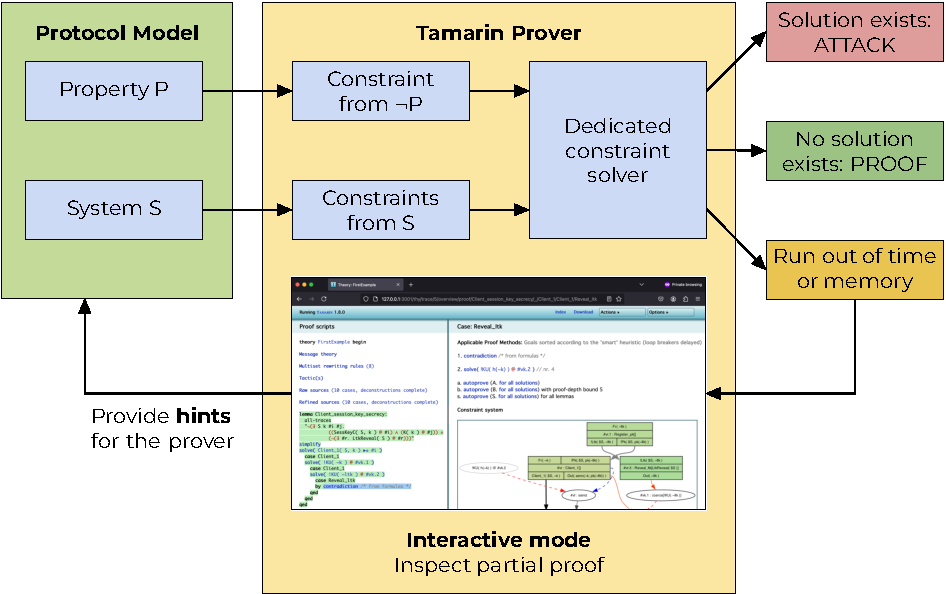
\includegraphics[width=.8\textwidth]
            {./figures/lecture_4/tamarin_workflow_8}%
    \end{figure}
\end{frame}

\begin{frame}[fragile]{Recap: Finding traces}
    \begin{table}[]
        \footnotesize
        \begin{tabular}{ll}
            MSR & Alternative syntax \\
            \toprule
            \begin{lstlisting}[style=tamarin, gobble=16]
                rule r1:
                  [ Fr(a), Fr(b), Fr(c) ]
                --[ Initialize(a, b, c) ]->
                  [ St_1(a, b, c), Out(a) ]
            \end{lstlisting} &
            $\mathrm{\dfrac{Fr(a) \quad Fr(b) \quad Fr(c)}{St\_1(a, b, c) \quad Out(a)}[\;Initialize(a, b, c)\;]}$ \\
            \midrule
            \begin{lstlisting}[style=tamarin, gobble=16]
                rule r2:
                  [ St_1(a, b, c), Fr(d) ]
                --[ Step(a, b, c, d) ]->
                  [ St_2(a, c, d), Out(c) ]
            \end{lstlisting} &
            $\mathrm{\dfrac{St\_1(a, b, c) \quad Fr(d)}{St\_2(a, c, d) \quad Out(c)}[\;Step(a, b, c, d)\;]}$ \\
            \midrule
            \begin{lstlisting}[style=tamarin, gobble=16]
                rule r3:
                  [ St_2(a, c, d), In(<a, c>) ]
                --[ Finish(a, c, d, c) ]->
                  [ !St(a, c, d) ]
            \end{lstlisting} &
            $\mathrm{\dfrac{St\_2(a, c, d) \quad In(\langle a, c \rangle)}{!St(a, c, d)}[\;Finish(a, c, d, c)\;]}$ \\
            \bottomrule \\
            \begin{lstlisting}[style=tamarin, gobble=16]
                // Finish(a,c,d,c) is reachable
                lemma trace: exists-trace
                    " Ex a c d #i .
                        Finish(a, c, d, c)@i "
            \end{lstlisting} &
            $\exists a, c, d (Finish(a,c,d,c))$
        \end{tabular}
    \end{table}
\end{frame}

\begin{frame}[fragile]{Recap: Dependency graphs}
    \begin{columns}[T]
        \begin{column}{0.5\textwidth}
            \begin{figure}
                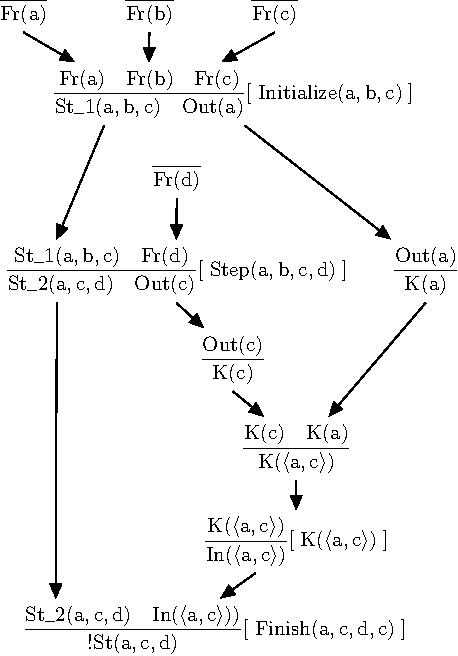
\includegraphics[width=.65\textwidth]
                    {./figures/lecture_5/dependency_graph}%
            \end{figure}
        \end{column}
        \begin{column}{0.5\textwidth}
            \begin{figure}
                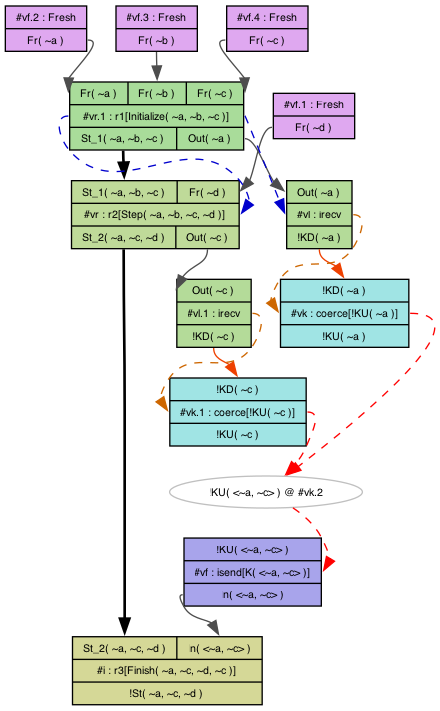
\includegraphics[width=.6\textwidth]
                    {./figures/lecture_5/dependency_graph_tamarin}%
            \end{figure}
        \end{column}
    \end{columns}
\end{frame}

\begin{frame}[fragile]{This lecture}
    \tableofcontents
\end{frame}

% ---------------------------------------------------------------------------- %

\section{Constraint Solving}

% ---------------------------------------------------------------------------- %

\begin{frame}[fragile]{Constraint solving}
    Given a set of \textbf{rules} $R$ and a \textbf{property} $P:$
    \begin{itemize}
        \item If the property is \textit{all-traces} (the default):
            \begin{itemize}
                \item Consider a set of constraints that represent
                      ($R$ and $\neg P$)
                \item No solution is proof of $P$
                \item Solutions are \textbf{counterexamples}
            \end{itemize}
        \item If the property is \textit{exists-trace}:
            \begin{itemize}
                \item Consider a set of constraints that represent ($R$ and $P$)
                \item No solution means that $P$ does not hold
                \item Solutions are witnesses that $P$ holds for some trace
            \end{itemize}
    \end{itemize}
\end{frame}

\begin{frame}[fragile]{Constraint solving}
    \begin{enumerate}
        \item \textbf{Precomputation for rules}
            \begin{itemize}
                \item Using static analysis, try to infer which rules must 
                      precede others
                \item Compute \textit{sources} for facts in the protocol
                \item Finite process
            \end{itemize}
        \item \textbf{Constraint solving}
            \begin{itemize}
                \item Backwards reachability analysis, searching for traces
                \item Constraint solving with formula and graph constraints
                \item Build a dependency graph to represent protocol executions
                \item Solved forms have a solution corresponding to an attack 
                      trace
                \item May not terminate
            \end{itemize}
    \end{enumerate}
\end{frame}

\begin{frame}[fragile]{Tamarin's constraint solving algorithm}
    \begin{algorithmic}[1]
        \Function{\textsc{Solve}}{$P \vDash_E \varphi$}
            \State $\hat{\varphi} \gets \neg \varphi$ rewritten into negation normal form
            \State $\Omega \gets \{\{\hat{\varphi}\}\}$
            \While{$\Omega \neq \varnothing$ and $\mathit{solved}(\Omega) = \varnothing$}
                \State choose $\Gamma$ $\rightsquigarrow_P \{\Gamma_1, \dots, \Gamma_k\}$ such that $\Gamma \in \Omega$
                \State $\Omega \gets (\Omega \smallsetminus \{\Gamma\}) \cup \{\Gamma_1, \dots, \Gamma_k\}$
            \EndWhile
            \If{$\mathit{solved}(\Omega) \neq \varnothing$}
                \State \textbf{return} "attack(s) found: ", $\mathit{solved}(\Omega)$
            \Else
                \State \textbf{return} "verification successful"
            \EndIf
            \EndFunction
    \end{algorithmic}
\end{frame}

\begin{frame}[fragile]{Constraint reduction}
    \begin{itemize}
        \item A \textbf{constraint reduction} rule transforms a constraint 
              system into a set of constraints systems
        \begin{equation*}
            \Gamma \rightsquigarrow \{\Gamma_1, \dots, \Gamma_{\mathrm{k}}\}
        \end{equation*}
        \vspace*{-.5cm}
        \item The relation is defined by a set of \textbf{reduction rules}
        \begin{itemize}
            \item Logical rules work on formula constraints
            \item Graph rules work on node and edge constraints
        \end{itemize}
        \item Every constraint reduction rule is \textit{sound} and
              \textit{complete}, i.e., it preservers the set of solutions
        \item However, the problem is \textbf{undecidable}; we cannot guarantee 
              termination!
    \end{itemize}
\end{frame}

\begin{frame}[fragile]{(Some) Constraint solving rules}
    \textbf{Trace formula reduction}
    \begin{table}
        \raggedright
        \footnotesize
        \begin{tabular}{lll}
            $\mathbf{s_{\approx}:}$
                & $\Gamma \rightsquigarrow_P\;\parallel_{\sigma \in \mathit{unify}_{AC}(t_1, t_2)}(\Gamma\sigma)$
                & if $(t_1 \approx t_2) \in \Gamma$ and $t_1 \neq_{AC} t_2$\\
            $\mathbf{s_{\doteq}:}$
                & $\Gamma \rightsquigarrow_P\;\Gamma\{i/j\}$
                & if $(i \doteq j) \in \Gamma$ and $i \neq j$\\
            $\mathbf{s_{@}:}$
                & $\Gamma \rightsquigarrow_P\;\parallel_{ri \in \lceil P \rceil^{DH}\cup\{\textsc{Isend}\}} \parallel_{f' \in \mathit{acts(ri)}}(i:ri, f \approx f', \Gamma)$
                & if $(f@i) \in \Gamma$ and $(f@i) \notin_{AC} as(\Gamma)$\\
            $\mathbf{s_{\perp}:}$
                & $\Gamma \rightsquigarrow_P\; \perp$
                & if $\perp \in \Gamma$\\
            $\mathbf{s_{\neg,\approx}:}$
                & $\Gamma \rightsquigarrow_P\; \perp$
                & if $\neg (t \approx t) \in_{AC} \Gamma$\\
            $\mathbf{s_{\neg,\doteq}:}$
                & $\Gamma \rightsquigarrow_P\; \perp$
                & if $\neg(i \doteq i) \in \Gamma$\\
            $\mathbf{s_{\neg,@}:}$
                & $\Gamma \rightsquigarrow_P\; \perp$
                & if $\neg(f@i) \in \Gamma$ and $(f@i) \in as(\Gamma)$\\
            $\mathbf{s_{\neg,\lessdot}:}$
                & $\Gamma \rightsquigarrow_P\; (i \lessdot j, \Gamma) \parallel (\Gamma\{i/j\})$
                & if $\neg(j \lessdot i) \in \Gamma$ and neither $i \lessdot_{\Gamma} j$ nor $i = j$\\
            $\mathbf{s_{\vee}:}$
                & $\Gamma \rightsquigarrow_P\; (\phi_1, \Gamma) \parallel (\phi_2, \Gamma)$
                & if $(\phi_1 \vee \phi_2) \in_{AC} \Gamma$ and $\{\phi_1, \phi_2\} \cap_{AC} \Gamma = \varnothing $\\
            $\mathbf{s_{\wedge}:}$
                & $\Gamma \rightsquigarrow_P\; (\phi_1, \phi_2, \Gamma)$
                & if $(\phi_1 \wedge \phi_2) \in_{AC} \Gamma$ and not $\{\phi_1, \phi_2\} \subseteq_{AC} \Gamma$
        \end{tabular}
    \end{table}
\end{frame}

% ---------------------------------------------------------------------------- %

\section{Proof Methods}

% ---------------------------------------------------------------------------- %

\begin{frame}[fragile]{Proof trees}
    \begin{itemize}
        \item Tamarin uses constraint solving to prove or disprove lemmas, 
              where each constraint reduction step generates one or more new 
              constraint systems
        \item This leads to a \textbf{proof tree}, which is visible in the GUI, 
              or output when Tamarin is run on the command line
        \item There can be any number of ``cases'' (including zero), which must 
              be resolved
        \item The \textbf{qed} symbol marks the end of a list of cases
    \end{itemize}
\end{frame}

\begin{frame}[fragile]{Proof methods}
    \begin{columns}[T]
        \begin{column}{0.55\textwidth}
            \vspace*{.25cm}
            \begin{lstlisting}[
                style=prooftree,
                gobble=16,
                mathescape=true,
            ]
                lemma trace:
                  exists-trace
                  "(*@\textcolor[HTML]{921C12}{$\exists$}@*) a b #i. Action(a,b) @ #i"
                (*@\alt<3->{\textbf{\textcolor[HTML]{2639B0}{simplify}}}{\textbf{by \textcolor[HTML]{2639B0}{sorry}}}@*)(*@\pause\pause@*)
                solve<<( Fact ( t1, t2 ) $\blacktriangleright$ #i1 )>>
                  case Fact_1(*@\pause@*)
                  solve<<( !KU( t1 ) @ #vk )>>
                    case Fact_2(*@\pause@*)
                    solve<<( (#i < #j) (*@\textcolor[HTML]{921C12}{$\parallel$}@*) (#j < #i) )>>
                      case case_1(*@\pause@*)
                      solve<<( splitEqs(i) )>>
                        case r_1(*@\pause@*)
                        solve<<( (#vl,0) ~~> (#vk,0) )>>
                          case r_2(*@\pause@*)
                          (*@\alt<7->{\textbf{by \textcolor[HTML]{2639B0}{contradiction}} \textcolor[HTML]{808080}{/* cyclic */}}{\textbf{by \textcolor[HTML]{2639B0}{sorry}}}@*)
                        next
                          case r_3(*@\pause@*)
                          (*@\alt<7->{\textbf{\textcolor[HTML]{2639B0}{SOLVED}} \textcolor[HTML]{808080}{// trace found}}{\textbf{by \textcolor[HTML]{2639B0}{sorry}}}@*)
                      qed
                    qed
                  qed
                qed
            \end{lstlisting}
        \end{column}
        \onslide<*>
        \begin{column}{0.45\textwidth}
            \begin{onlyenv}<1>
                \begin{tcolorbox}[
                    title = {\fontfamily{pcr}\fontseries{b}\selectfont sorry},
                    left = 1mm,
                    top = 1mm,
                    right = 1mm,
                    bottom = 1mm,
                ]
                    Special ``proof method'' that proves nothing. Used as a 
                    placeholder.
                \end{tcolorbox}
                Tamarin gives us several options to replace \texttt{sorry} with an actual proof:
                \begin{lstlisting}[
                    style=prooftree,
                    gobble=20,
                    mathescape=true,
                    numbers=none,
                    frame=single,
                ]
                    1. simplify
                    2. induction

                    a. autoprove
                    b. autoprove proof-depth bound 5
                    s. autoprove for all lemmas
                \end{lstlisting}
            \end{onlyenv}
            \begin{onlyenv}<2>
                \begin{tcolorbox}[
                    title = {\fontfamily{pcr}\fontseries{b}\selectfont simplify},
                    left = 1mm,
                    top = 1mm,
                    right = 1mm,
                    bottom = 1mm,
                ]
                    Translate a formula's negation into constraints. Typically 
                    the first step.
                \end{tcolorbox}
                \begin{tcolorbox}[
                    title = {\fontfamily{pcr}\fontseries{b}\selectfont induction},
                    left = 1mm,
                    top = 1mm,
                    right = 1mm,
                    bottom = 1mm,
                ]
                    Prove a lemma using induction on the length of the trace. 
                    Only possible as the first proof step.
                \end{tcolorbox}
            \end{onlyenv}
            \begin{onlyenv}<3>
                \begin{tcolorbox}[
                    title = {\small Premise constraints\hfill(line 5)},
                    left = 1mm,
                    top = 1mm,
                    right = 1mm,
                    bottom = 1mm,
                ]
                    Find the origin of facts from protocol rules.
                \end{tcolorbox}
            \end{onlyenv}
            \begin{onlyenv}<4>
                \begin{tcolorbox}[
                    title = {\small Action constraints\hfill(line 7)},
                    left = 1mm,
                    top = 1mm,
                    right = 1mm,
                    bottom = 1mm,
                ]
                    Solve formula constraints, such as action fact requirements 
                    or intruder detection constraints.
                \end{tcolorbox}
            \end{onlyenv}
            \begin{onlyenv}<5>
                \begin{tcolorbox}[
                    title = {\small Disjunction\hfill(line 9)},
                    left = 1mm,
                    top = 1mm,
                    right = 1mm,
                    bottom = 1mm,
                ]
                    Turn a disjunction inside a formula into a case distinction 
                    at the constraint system level.
                \end{tcolorbox}
            \end{onlyenv}
            \begin{onlyenv}<6>
                \begin{tcolorbox}[
                    title = {\small Equation split\hfill(line 11)},
                    left = 1mm,
                    top = 1mm,
                    right = 1mm,
                    bottom = 1mm,
                ]
                    Perform a case split on different possible substitutions.
                \end{tcolorbox}
            \end{onlyenv}
            \begin{onlyenv}<7>
                \begin{tcolorbox}[
                    title = {\small Deconstruction chain (line 13)},
                    left = 1mm,
                    top = 1mm,
                    right = 1mm,
                    bottom = 1mm,
                ]
                    Compute whether the adversary can extract a given term from 
                    some message.
                \end{tcolorbox}
            \end{onlyenv}
            \begin{onlyenv}<8>
                \begin{tcolorbox}[
                    title = {\fontfamily{pcr}\fontseries{b}\selectfont contradiction},
                    left = 1mm,
                    top = 1mm,
                    right = 1mm,
                    bottom = 1mm,
                ]
                    Tamarin has found a contradiction to the current 
                    constraint system. For example, circular dependencies or 
                    formulas evaluating to false. This means that there is no 
                    solution for the current constraint system.
                \end{tcolorbox}
            \end{onlyenv}
            \begin{onlyenv}<9>
                \begin{tcolorbox}[
                    title = {\fontfamily{pcr}\fontseries{b}\selectfont SOLVED},
                    left = 1mm,
                    top = 1mm,
                    right = 1mm,
                    bottom = 1mm,
                ]
                    Tamarin has solved the constraint system; no more proof 
                    methods are applicable. Typically means that we have found 
                    an attack.
                \end{tcolorbox}
            \end{onlyenv}
        \end{column}
    \end{columns}
\end{frame}

\begin{frame}[fragile]{Proof method annotations}
    The list of currently available proof methods can have annotations:
    \begin{itemize}
        \item An action constraint is \textbf{currently deducible} when it is 
              composed only from public constants and does not contain private 
              function symbols, or when it can be extracted from a sent message 
              using only unpairing or inversion
        \item An action constraint is \textbf{probably constructible} when it 
              concerns a message that does not contain a fresh name or a fresh 
              variable, and therefore can likely be constructed by the adversary
        \item An action constraint is \textbf{useful} when it appears in 
              specific ways in the formulas of the constraint system
    \end{itemize}
\end{frame}

\begin{frame}[fragile]{Avoiding loops}
    \begin{itemize}
        \item To avoid loops when solving premise constraints, Tamarin computes 
              a set of premises, called \textbf{loop breakers}
        \item Idea: Consider a graph containing a node for each rule, and an 
              edge between two rules, if the second one has a premise fact that 
              is part of the conclusion facts of the first one
        \item This graph over-approximates possible sequences of rules; any 
              potential looping sequence of rule instances will show up as a 
              \textbf{cycle}
        \item The goal is then to \textbf{remove a minimal set of premises} 
              (the loop breakers) so that the remaining graph has no cycles
        \item Not a unique set; Tamarin might not find the ``optimal'' solution
    \end{itemize}
\end{frame}

\begin{frame}[fragile]{Heuristics}
    \begin{itemize}
        \item Tamarin uses \textbf{heuristics} to decide which proof method to 
              apply
        \item These play an important role in whether Tamarin terminates and, 
              if it does, how quickly (i.e., its efficiency)
        \item Heuristics have no influence on the result's correctness;
              \textbf{any} conclusion obtained by Tamarin is
              \textbf{always correct}
        \item The default options is the \textit{smart} heuristic
        \begin{itemize}
            \item Works well on many examples
            \item Prioritizes chain constraints, disjunctions, premise 
                  constraints, action constraints, and adversary knowledge that 
                  includes private or fresh terms (in this order)
            \item \textit{Probably constructible} and
                  \textit{currently deducible} constraints are assigned lower 
                  priority and loop breakers are delayed
        \end{itemize}
    \end{itemize}
\end{frame}

% ---------------------------------------------------------------------------- %
% Reading Material
% ---------------------------------------------------------------------------- %
\setbeamertemplate{frametitle continuation}{}

\begin{frame}[fragile,allowframebreaks]{Reading material}
    \textbf{Recommended reading}:\\ \;
        ~\cite[Ch. 6.6--6.8]{tamarin-book},
        ~\cite[Ch. 8.3--8.4]{meier2013thesis},
        ~\cite{schmidt2012tamarin}
    \begin{refsection}
        \nocite{tamarin-book, meier2013thesis, schmidt2012tamarin}
        \printbibliography[heading=none]
    \end{refsection}
\end{frame}

\begin{frame}[fragile]{Additional reading}
    \textbf{Additional reading}:
        ~\cite{comon-lundh2005finite},
        ~\cite{santiago2008finite}
    \begin{refsection}
        \nocite{comon-lundh2005finite, santiago2008finite}
        \printbibliography[heading=none]
    \end{refsection}
\end{frame}
% ---------------------------------------------------------------------------- %

\end{document}
